\chapter{Manual do Usuário}\label{chap:user-manual-appendix}
Este apêndice contém um manual básico do usuário, mostrando a navegação em algumas telas e elucidando os fluxos de interação com o sistema para os três perfis básicos de usuário: Aluno, Professor/Convidado e Coordenador.

O sistema foi construído usando Django na versão 2.1, roda com um banco de dados (que pode ser SQLite ou PostgreSQL, dependendo do ambiente) e com uma instância do Redis para cache (em especial para suporte do Select2). Para hospedar os arquivos, foi usado o Google Drive. Por fim, para o front-end, foi usado como auxilio o MDBootstrap e também o JQuery. Todas as telas foram construídas pensando na navegação mobile, o que permite que todas as instruções deste manual sejam executadas em \textit{smartphones} sem maiores problemas.

Para entender melhor a navegação no sistema, as funcionalidades serão divididas em três grandes grupos:

\begin{itemize}
    \item Alunos: Podem verificar seus grupos de trabalho e suas disciplinas inscritas, bem como as atividades em aberto e realizar submissões delas. Podem ver também parte dos resultados das revisões das submissões.
    \item Professores/Convidados: Possuem maior poder no sistema, podendo ver todas as disciplinas e os grupos de trabalho que são coordenadores. Podem realizar as revisões das entregas dos alunos, como também podem avaliar os projetos em que foram alocados nos eventos.
    \item Coordenadores: Possuem plenos poderes no sistema, podendo gerenciar todos os recursos existentes.
\end{itemize}

\section{Aluno}
\begin{figure}[H]
    \centering
    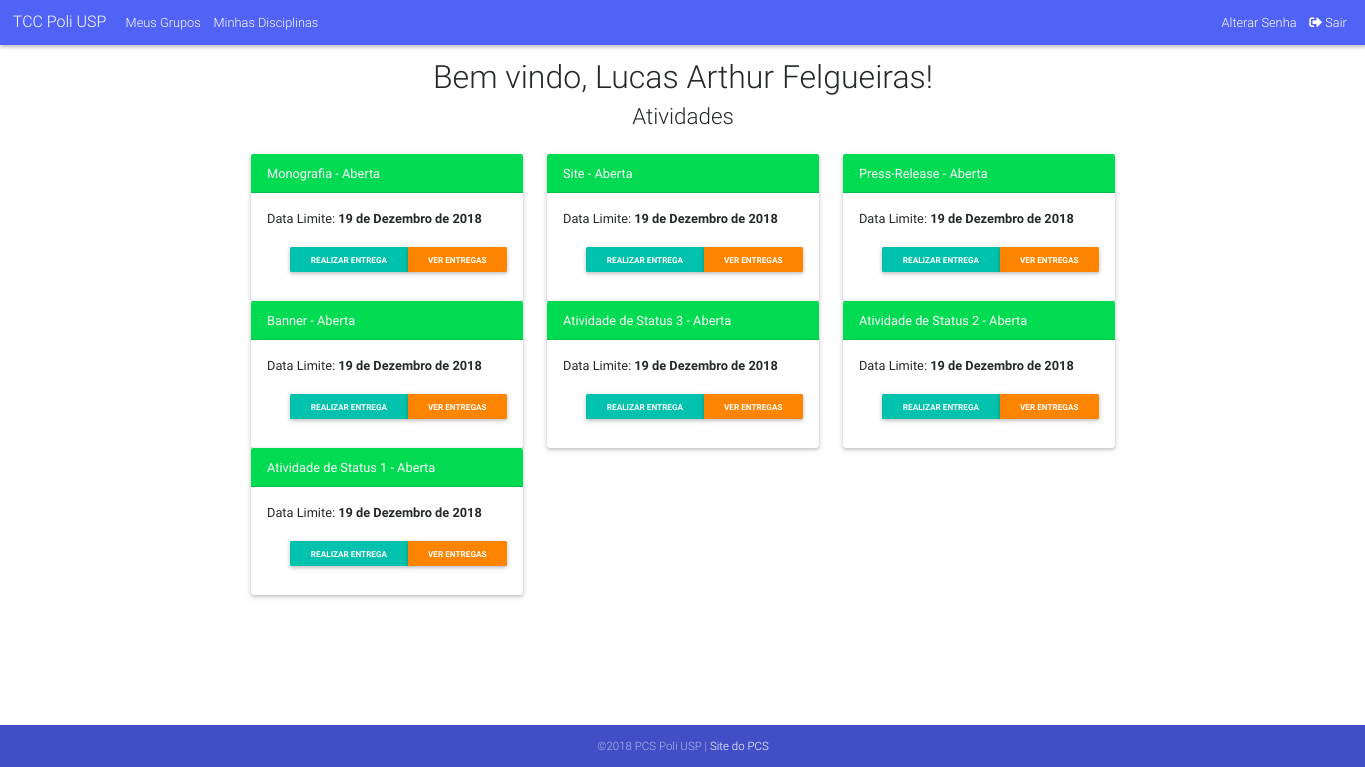
\includegraphics[scale=0.3]{imagens/tela_inicial_aluno.png}
    \caption{Tela Inicial do Aluno}
    \label{fig:initial-screen-student}
\end{figure}

Na tela inicial de aluno, são exibidas as atividades da disciplina as quais o aluno participa. No menu superior, há as opções de ver os grupos de trabalho onde participa e as disciplinas em que está cadastrado.

\subsection{Tela Inicial}
Para cada atividade listada na tela inicial, é possível ver as entregas já realizadas pelo seu grupo ao selecionar \textbf{Ver Entregas}. Na listagem das entregas da atividade escolhida, é possível ver cada entrega com mais detalhes (ao selecionar \textbf{Ver Mais}, alterar detalhes da entrega (caso não tenha sido avaliada) ao selecionar \textbf{Editar}, bem como realizar novas entregas ao selecionar \textbf{Nova Entrega}.

Também é possível, na própria tela inicial, realizar uma entrega para uma atividade da lista, ao selecionar \textbf{Realizar Entrega}. Cada entrega alerta, por e-mail, os orientadores/co-orientadores. Vale lembrar que entregas podem ocorrer enquanto a atividade estiver aberta e edições às entregas apenas quando ela não tiver sido avaliada.

\subsection{Meus Grupos}
Entrando na parte de \textbf{Meus Grupos}, é possível ver todos os grupos de trabalho em que o próprio aluno está inscrito. Selecionando o ícone de \faEye, é possível ver mais detalhes do grupo, como a participação dos orientadores, o nome do projeto, entre outros.

\subsection{Minhas Disciplinas}
Já na parte de \textbf{Minhas Disciplinas}, é possível ver detalhes das disciplinas em que o aluno está inscrito, selecionando o ícone de \faEye na disciplina desejada, ou ver as atividades da disciplina selecionando o ícone de \faListUl. Dentro da listagem de atividades, o procedimento de navegação é o mesmo citado anteriormente, para ver detalhes, realizar e editar submissões.

\section{Professor/Convidado}
\begin{figure}[H]
    \centering
    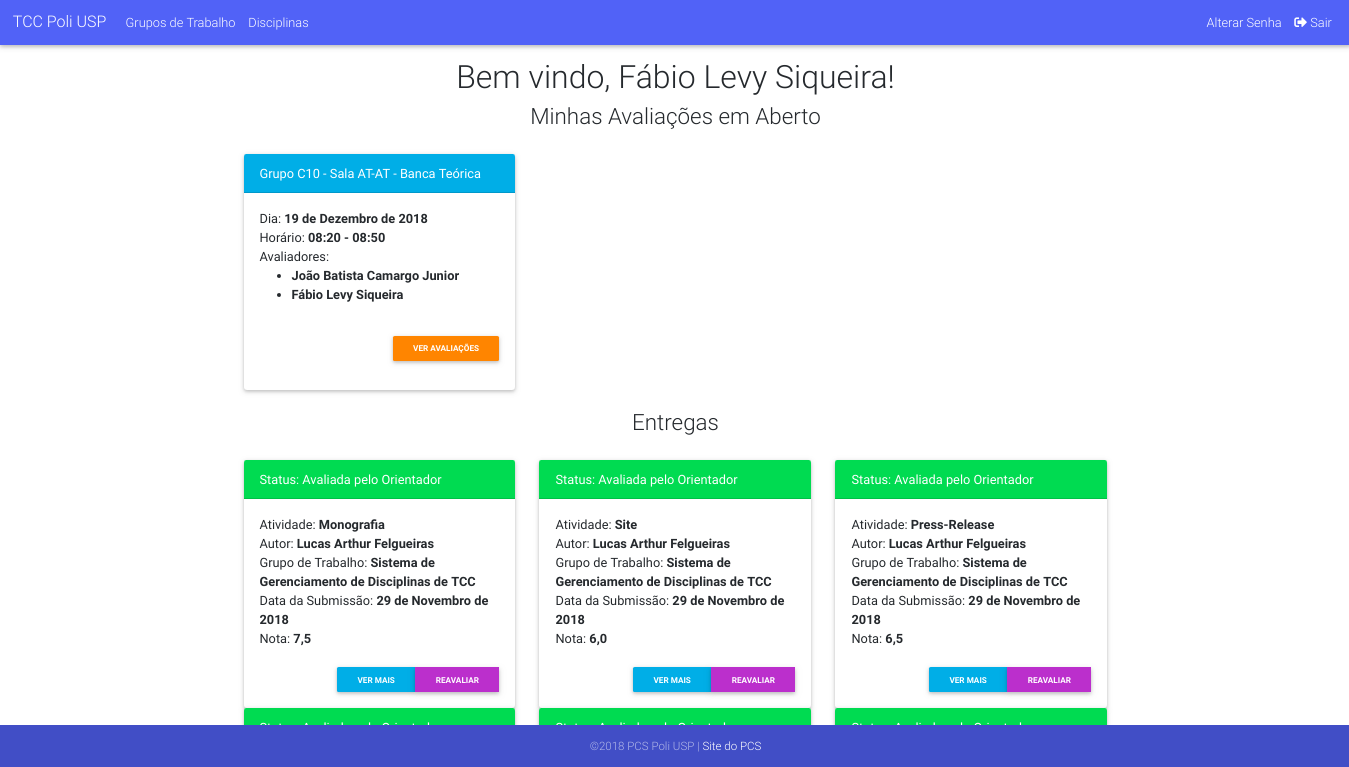
\includegraphics[scale=0.3]{imagens/tela_inicial_professor.png}
    \caption{Tela Inicial do Professor/Convidado}
    \label{fig:initial-screen-staff}
\end{figure}

Já na tela inicial de professor/convidado, são exibidas as informações pertinentes às submissões dos grupos de trabalho em quem é orientador/co-orientador, além dos eventos em que foram alocados como avaliadores teóricos ou práticos. No menu, é possível ver todas as disciplinas existentes no sistema, como também ver todos os grupos de trabalho em que está incluso.

\subsection{Tela Inicial}
Na tela inicial, a parte de avaliações se assemelha a do aluno, com o diferencial que a listagem é de submissões de atividades. Para cada atividade, é possível ver mais detalhes ao selecionar \textbf{Ver Mais}, como também realizar a avaliação selecionando \textbf{Avaliar} ou \textbf{Reavaliar}, de acordo com o estado da submissão. Vale lembrar que, caso seja um co-orientador, não é possível editar a avaliação feita por um orientador.

Já a parte de eventos, é possível ver quais eventos o indivíduo irá participar, qual o tipo do evento, o grupo relacionado, outros avaliadores, a sala, o dia e o horário correspondentes. Para ver as avaliações do grupo, basta selecionar \textbf{Ver Avaliações}.

\begin{figure}[H]
    \centering
    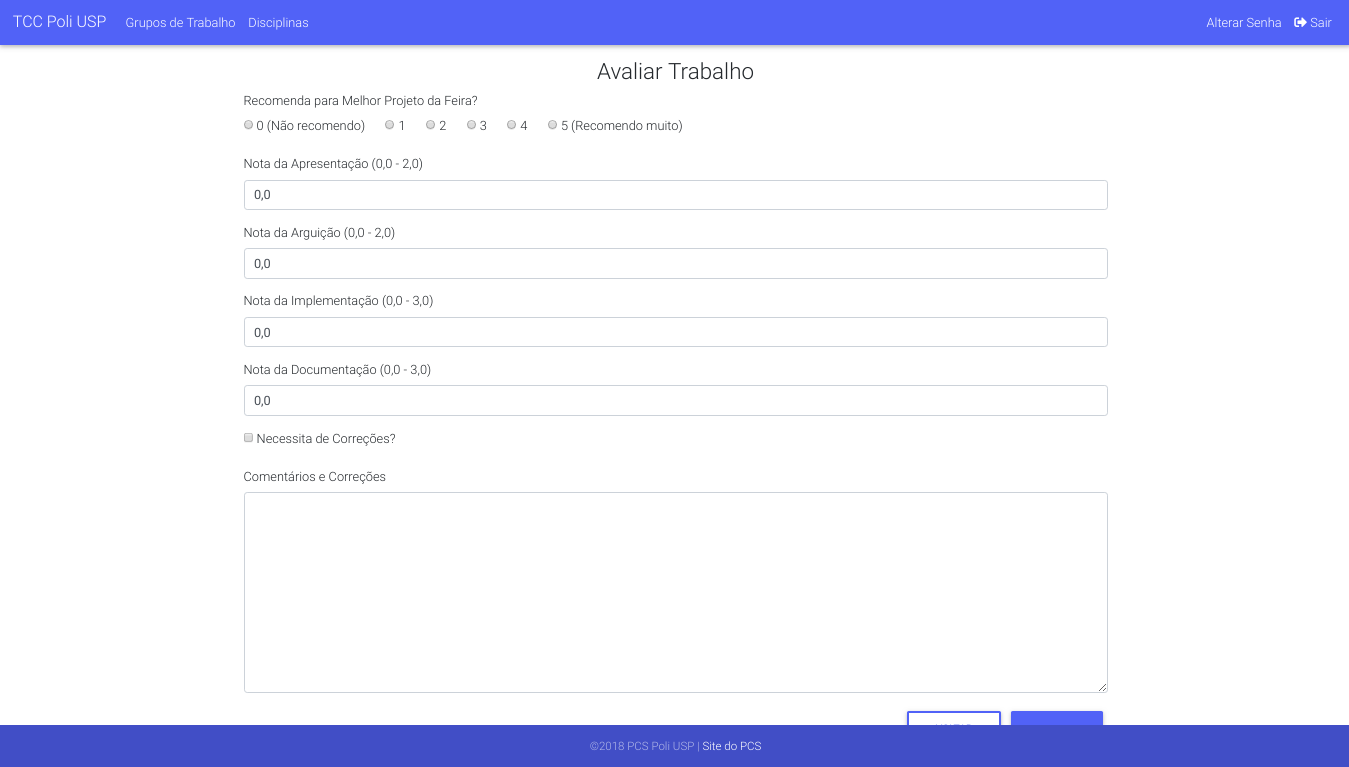
\includegraphics[scale=0.3]{imagens/tela_nova_avaliacao.png}
    \caption{Tela de Nova Avaliação Teórica}
    \label{fig:evaluations-new}
\end{figure}

Na tela de avaliações, apenas as próprias avaliações serão exibidas (caso o docente/convidado não seja também o coordenador da disciplina). Para realizar uma nova avaliação, basta selecionar \textbf{Nova Avaliação}. A avaliação ainda é editável, ao selecionar \textbf{Editar}, porém apenas enquanto o evento estiver acontecendo, pois ao término do evento, as avaliações não são mais editáveis.

\subsection{Grupos de Trabalho}
Entrando na parte de \textbf{Grupos de Trabalho}, é possível ver todos os grupos de trabalho em que o próprio professor/convidado está inscrito. Semelhante ao comportamento dos alunos, selecionando o ícone de \faEye, é possível ver mais detalhes do grupo, como a participação dos orientadores, o nome do projeto, entre outros.
Além dessa funcionalidade, há também a confirmação de participação, selecionando \textbf{Confirmar Participação} no grupo desejado.

\subsection{Disciplinas}
Já na parte de \textbf{Disciplinas}, é possível ver detalhes de todas as da disciplina, também selecionando o ícone de \faEye, ou ver as atividades de uma disciplina específica selecionando o ícone de \faListUl. Dentro da listagem de atividades, é possível ver também, para cada uma, as entregas realizadas dos grupos em que orienta, ao selecionar \textbf{Ver Entregas}. A listagem de entregas é semelhante a que foi comentada anteriormente na tela inicial, permitindo avaliações e detalhes maiores de cada entrega submetida.

\section{Coordenador}
\begin{figure}[H]
    \centering
    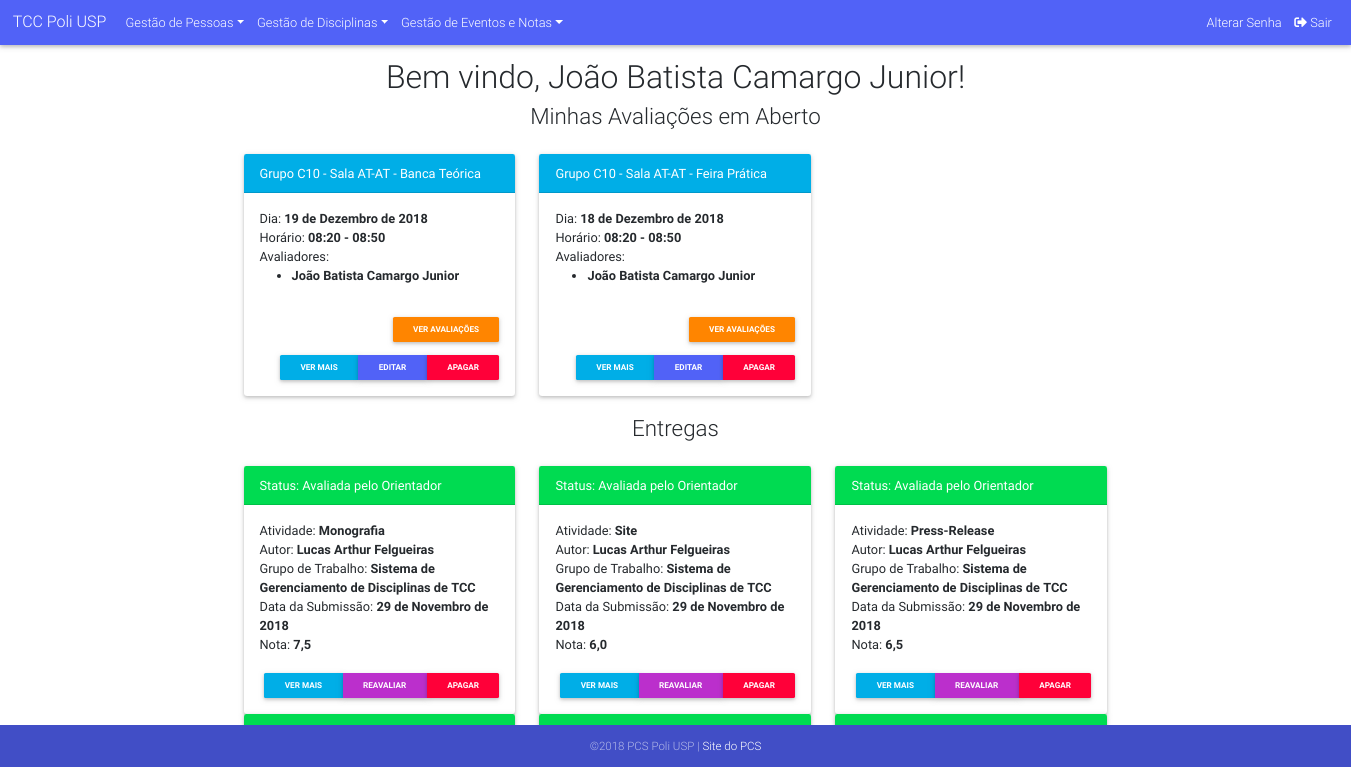
\includegraphics[scale=0.3]{imagens/tela_inicial_coordenador.png}
    \caption{Tela Inicial do Coordenador, com permissões de Professor}
    \label{fig:initial-screen-coordinator}
\end{figure}

A tela inicial de coordenador, em geral, não costuma ter nada, além do menu inicial. Como a aplicação permite múltiplos perfis, os coordenadores da disciplina também podem orientar grupos e avaliar projetos como um docente comum. Logo, a tela inicial corresponde a mesma do docente/convidado. Se, futuramente, um coordenador novo for cadastrado e ele não estiver na lista de docentes ou de convidados, a tela inicial terá apenas a mensagem de boas vindas.

\subsection{Gestão de Pessoas}
Ao selecionar \textbf{Gestão de Pessoas}, surgem três opções, todas relacionadas à usuários: \textbf{Docentes}, \textbf{Alunos} e \textbf{Convidados Externos}.

\subsubsection{Docentes}
Ao selecionar \textbf{Docentes}, surge toda a lista de docentes do sistema. Para cadastrar um docente, basta selecionar \textbf{Novo Docente}, enviando um e-mail com instruções de acesso ao novo docente no término do cadastro. Para gerenciar um docente existente, basta selecionar as opções: \faEye para ver mais, \faEdit para editar e \faTrash para excluí-lo.

\subsubsection{Alunos}
Ao selecionar \textbf{Alunos}, o comportamento é semelhante, com a lista de alunos do sistema. Para cadastrar um aluno, basta selecionar \textbf{Novo Aluno}, enviando um e-mail com instruções de acesso ao novo aluno no término do cadastro. Para gerenciar um aluno existente, basta selecionar as opções: \faEye para ver mais, \faEdit para editar e \faTrash para excluí-lo (lembrando que é impossível excluir seu próprio usuário).

\begin{figure}[H]
    \centering
    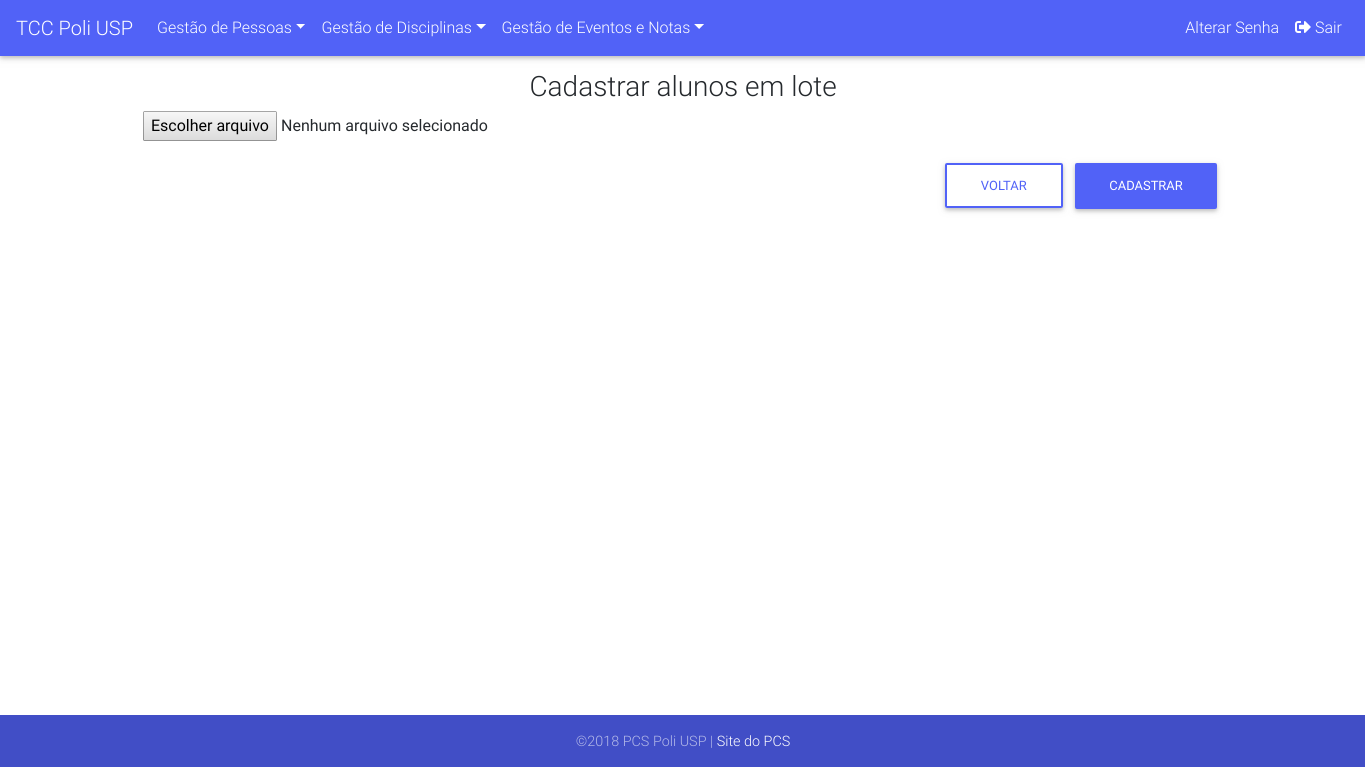
\includegraphics[scale=0.3]{imagens/tela_cadastro_massivo.png}
    \caption{Tela de Cadastro Massivo de Alunos}
    \label{fig:massive-sign-up}
\end{figure}

O diferencial desta parte está no cadastro massivo de alunos (usando como entrada a planilha de nomes gerada pelo JúpiterWeb). Ao selecionar \textbf{Cadastrar Alunos Massivamente}, será possível carregar a planilha e, para cada nome encontrado, ele será cadastrado e um e-mail com instruções será disparado. Ao término do cadastro, você será redirecionado à tela de cadastro de disciplinas, dado que é usual realizar o cadastro massivo na hora de cadastrar uma disciplina.

\subsubsection{Convidados Externos}
Por fim, ao selecionar \textbf{Convidados Externos}, surge toda a lista de convidados do sistema. Novamente, para cadastrar um convidado, basta selecionar \textbf{Novo Convidado Externo}, enviando um e-mail com instruções de acesso ao novo convidado no término do cadastro. Para gerenciar um convidado existente, basta selecionar as opções: \faEye para ver mais, \faEdit para editar e \faTrash para excluí-lo.

\subsection{Gestão de Disciplinas}
Já ao selecionar \textbf{Gestão de Disciplinas}, surgem duas opções relacionadas ao dia-a-da das disciplinas de formatura: \textbf{Disciplinas} e \textbf{Grupos de Trabalho}.

\subsubsection{Disciplinas}
Ao selecionar \textbf{Disciplinas}, o comportamento é bem semelhante ao dos outros perfis de usuário, porém listando todas as disciplinas. Para cadastrar uma nova disciplina, selecione \textbf{Nova Disciplina}, onde dentro do formulário há uma opção também para cadastro massivo de alunos (\textbf{Cadastrar Alunos Massivamente}). Para ver mais sobre uma em específico, basta selecionar o ícone de \faEye, para editá-la, o ícone de \faEdit, para apagá-la, \faTrash. Para ver as atividades de uma disciplina específica, deve-se selecionar o ícone de \faListUl.

Dentro da listagem de atividades, é possível cadastrar uma nova atividade em \textbf{Nova Atividade da Disciplina}. Para gerenciar uma atividade criada, basta selecionar a opção desejada: \textbf{Ver mais}, \textbf{Editar} ou \textbf{Apagar}. É possível ver também, para cada uma, as entregas realizadas de todos os grupos, ao selecionar \textbf{Ver Entregas}. A listagem de entregas é semelhante a que foi comentada anteriormente na tela inicial, permitindo avaliações (caso seja orientador/co-orientador) e detalhes maiores de cada entrega submetida.

\subsubsection{Grupos de Trabalho}
Agora, ao selecionar \textbf{Grupos de Trabalho}, a gestão é semelhante ao que foi comentado anteriormente, porém com a visualização de todos os grupos de trabalho. Para cadastrar um novo grupo, basta selecionar \textbf{Novo Grupo de Trabalho}, enviando e-mail para todos os envolvidos no final do cadastro. Selecionando o ícone de \faEye, é possível ver mais detalhes do grupo, selecionando \faEdit, é possível editá-lo, selecionando \faTrash, é possível apagá-lo. Se o coordenador estiver em um grupo de trabalho, também há a confirmação de participação no grupo ao selecionar \textbf{Confirmar Participação}.

\subsection{Gestão de Eventos e Notas}
A última seção do menu \textbf{Gestão de Eventos e Notas} possui três opções relacionadas aos eventos e notas finais: \textbf{Salas}, \textbf{Eventos} e \textbf{Fórmulas}.

\subsubsection{Salas}
\begin{figure}[H]
    \centering
    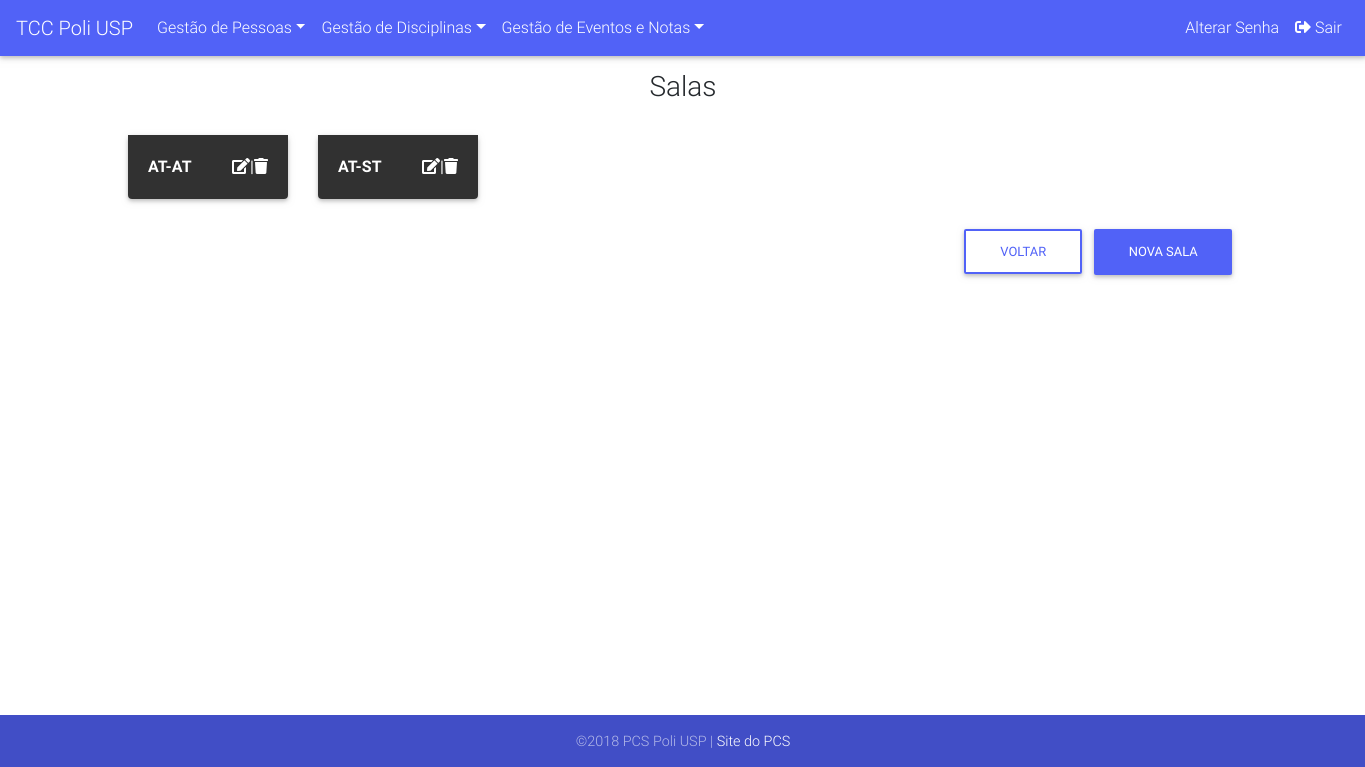
\includegraphics[scale=0.3]{imagens/tela_lista_salas.png}
    \caption{Tela de Listagem de Salas}
    \label{fig:rooms-list}
\end{figure}

Ao selecionar \textbf{Salas}, surge a lista de salas do sistema. Para cadastrar uma nova sala, basta selecionar \textbf{Nova Sala} e escolher as opções de bloco, andar e identificador. Para editar uma sala da listagem, selecione \faEdit, para apagar uma sala, \faTrash.

\begin{figure}[H]
    \centering
    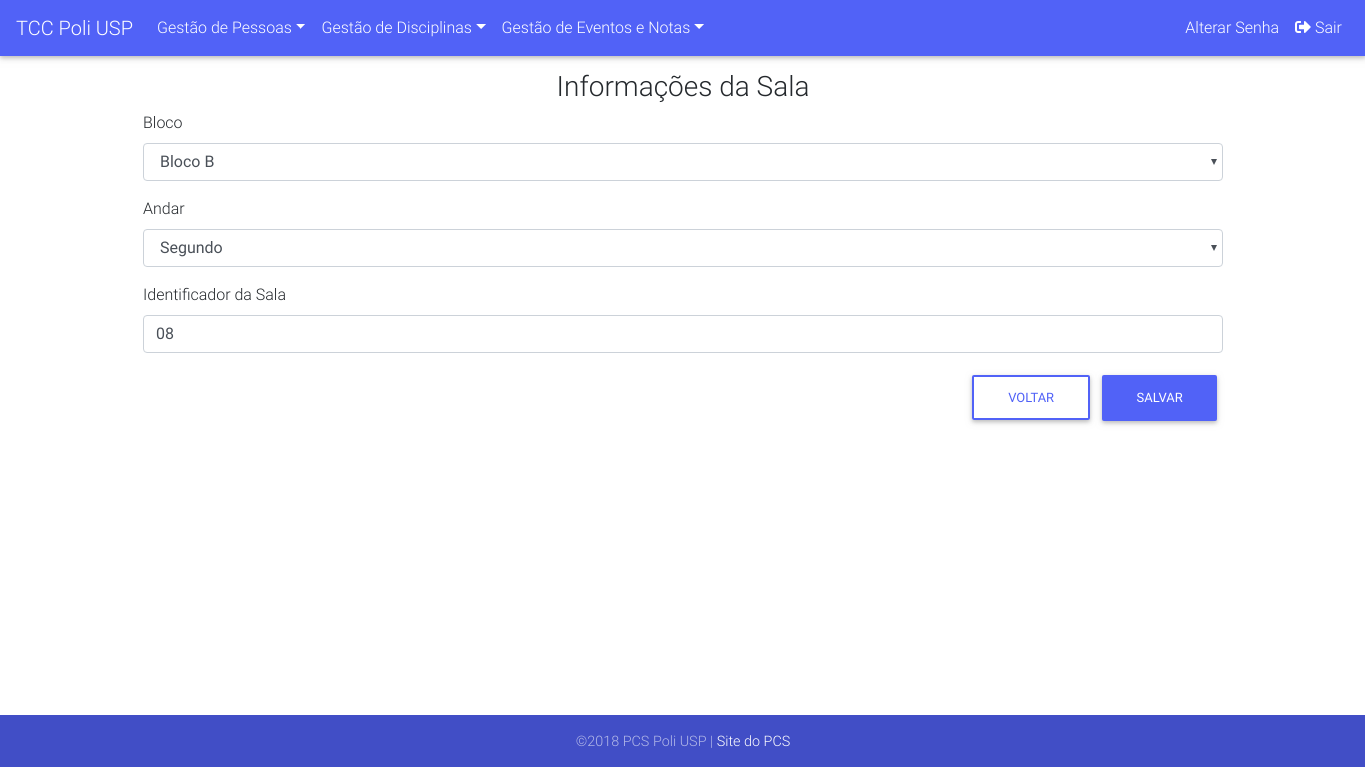
\includegraphics[scale=0.3]{imagens/tela_nova_sala.png}
    \caption{Tela de Nova Sala, cadastrando como exemplo a B2-08}
    \label{fig:rooms-new}
\end{figure}

\subsubsection{Eventos}
Agora, ao selecionar \textbf{Eventos}, surge a lista de eventos totais do sistema, tanto bancas teóricas como feiras práticas. Para cadastrar um novo evento, basta selecionar \textbf{Novo Evento}, lembrando que para cada evento são necessárias duas disciplinas: uma quadrimestral e outra semestral. Para cada evento, é possível realizar seu gerenciamento: \textbf{Ver mais}, \textbf{Editar} ou \textbf{Apagar}. E em cada evento, é possível alocar os grupos de trabalho que participarão da feira ou da banca, selecionando \textbf{Alocar Grupos}.

Na listagem de alocações de grupos, é possível ver todos os grupos alocados, com dia, horário, sala e avaliadores, permitindo seu gerenciamento com as opções: \textbf{Ver mais}, \textbf{Editar} ou \textbf{Apagar}. Para realizar uma nova alocação, basta selecionar \textbf{Nova Alocação} e informar os detalhes, lembrando que o horário deve estar dentro da janela do evento, bem como não deve ter nenhuma sala ocupada no horário desejado.

\begin{figure}[H]
    \centering
    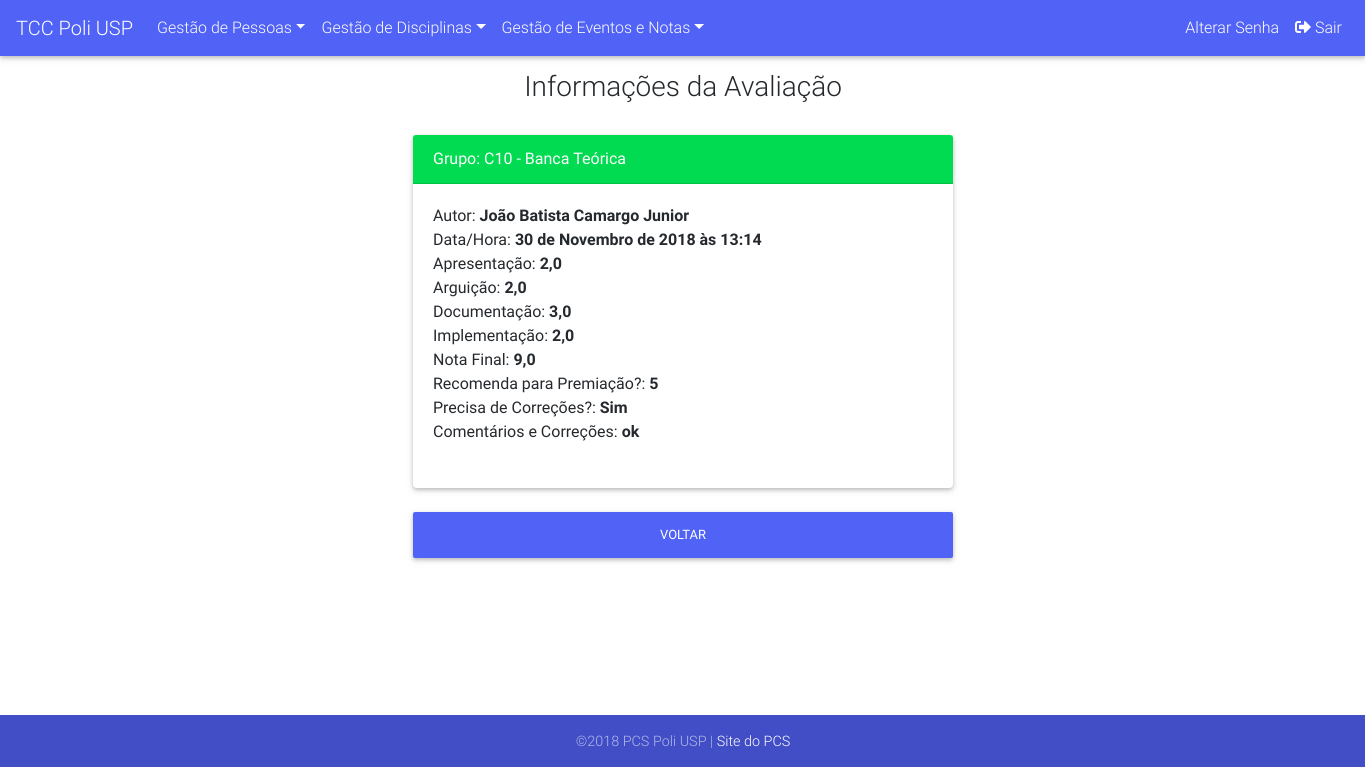
\includegraphics[scale=0.3]{imagens/tela_detalhes_avaliacao.png}
    \caption{Tela de Detalhes da Avaliação}
    \label{fig:evaluations-show}
\end{figure}

Em cada alocação, é possível ver as avaliações já realizadas, selecionando \textbf{Ver Avaliações}. Na listagem de avaliações, pode-se ver todas as avaliações do grupo e, para cada uma, é possível realizar seu gerenciamento: \textbf{Ver mais}, \textbf{Editar} ou \textbf{Apagar}, lembrando que as duas últimas opções são possíveis apenas se o coordenador estiver alocado para avaliar, podendo excluir e editar apenas sua avaliação.

\subsubsection{Fórmulas}
Por fim, ao selecionar \textbf{Fórmulas}, surge a lista de fórmulas totais. O conceito de fórmula consiste em juntar componentes de avaliação e, com base nelas, calculas as notas. As componentes da fórmula são: disciplina semstral, disciplina quadrimestral, banca teórica e feira prática. O cálculo geral é realizado da seguinte forma:

Sendo \begin{math}n\end{math} a quantidade de atividades:

\begin{equation}
    mediaAtividades = \frac{\sum_{i=1}^{n}(pesoAtv_{i}*notaAtv_{i})}{\sum_{i=1}^{n}(pesoAtv_{i})}
    \label{eq:activities}
\end{equation}

Sendo \begin{math}p\end{math} a quantidade de avaliadores práticos:

\begin{equation}
    mediaPratica = \frac{\sum_{k=1}^{p}(notaAvaliador_{k})}{p}
    \label{eq:practical}
\end{equation}

Sendo \begin{math}t\end{math} a quantidade de avaliadores teóricos (em geral são três):

\begin{equation}
    mediaTeorica = \frac{\sum_{j=1}^{t}(notaAvaliador_{j})}{t}
    \label{eq:theoretical}
\end{equation}

Por fim, a média final:

\begin{equation}
    mediaFinal = \frac{mediaAtividades + pesoBanca * mediaTeorica + pesoFeira * mediaPratica}{1 + pesoBanca + pesoFeira}
    \label{eq:final}
\end{equation}

Na hora de criar uma fórmula (selecionando \textbf{Nova Fórmula}), deve-se selecionar as disciplinas relacionadas para obter as atividades e os eventos para obter as notas dos avaliadores. Para calcular a média de atividades, apenas a última submissão revisada por orientador/co-orientador é levada em consideração para cada atividade. A vantagem de usar este método está na generalização do cálculo, tornando possível estabelecer fórmulas também para a primeira disciplina de TCC, permitindo eventos teóricos e práticos para a parte de especificação do projeto.

\begin{figure}[H]
    \centering
    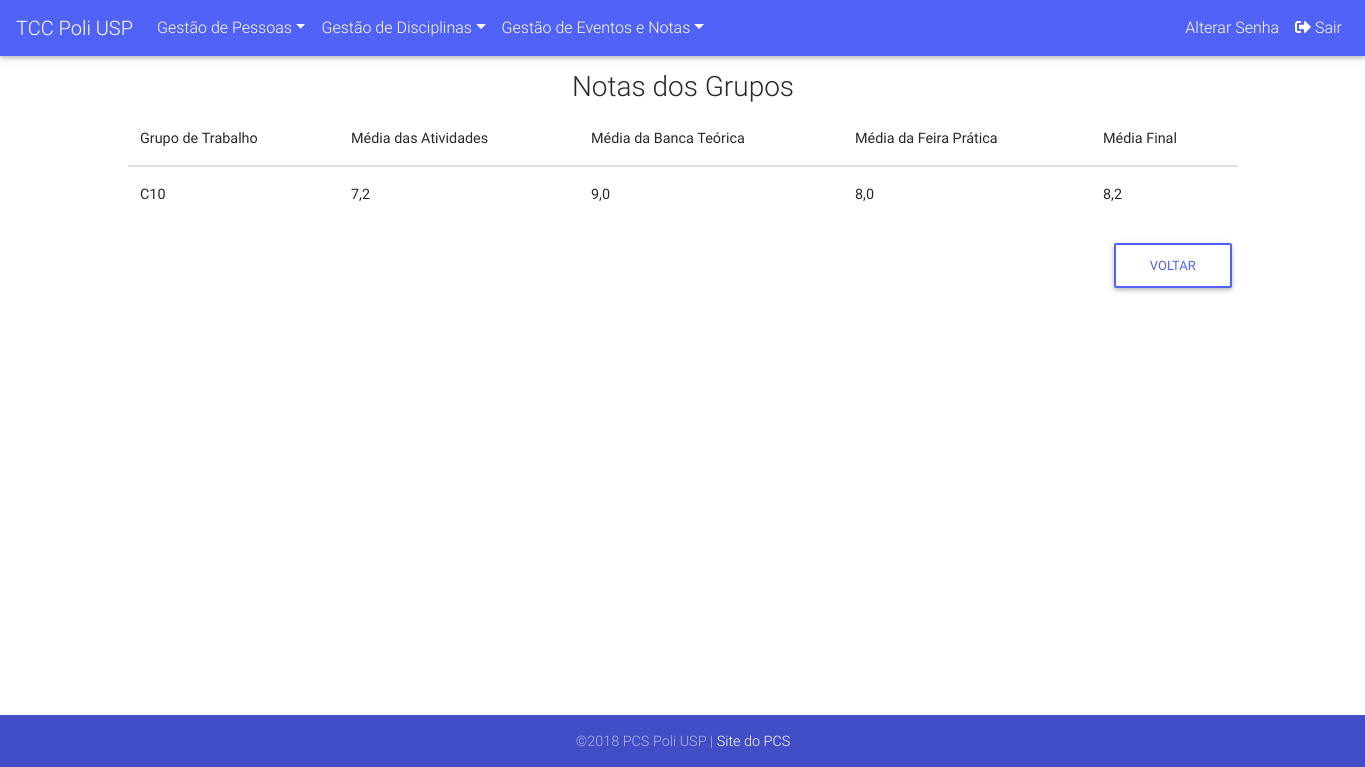
\includegraphics[scale=0.3]{imagens/tela_notas_calculadas.png}
    \caption{Tela de Notas Calculadas por Grupo de Trabalho}
    \label{fig:scores-list}
\end{figure}

Após salvar a nova fórmula, é possível realizar seu gerenciamento: ver mais selecionando \faEye, editar selecionando \faEdit e apagar selecionando \faTrash. Para efetuar o cálculo das notas com base nas fórmulas acima, selecione \faClockO. Após o cálculo, para ver as notas dos grupos, basta selecionas \faListUl. Em cada nota, há o grupo de trabalho relacionado, as componentes individuais e a média final. O cálculo pode ser refeito quantas vezes desejar, pois a cada novo cálculo a pontuação é recalculada e salva na componente do grupo de trabalho.

\section{Funcionalidades Comuns}
Para todos os perfis de usuário, há funcionalidades básicas e que são importantes para o funcionamento do sistema. São elas:

\subsection{Recuperar Senha}
No menu sem acessar o sistema, ao selecionar \textbf{Recuperar Senha}, a pessoa é redirecionada a um formulário onde, ao entrar com o e-mail, se ele estiver no sistema, ele recebe um e-mail com instruções para redefinir a senha, de acordo com as regras do formulário.

\subsection{Alterar Senha}
No menu, entrando no sistema, ao selecionar \textbf{Alterar Senha}, a pessoa é redirecionada a um formulário onde tem a possibilidade de redefinir a senha, inserindo a senha antiga e a nova senha, de acordo com as regras do formulário.